
\section{Hardware}

	A major component of the project was discovering what was available in the industry.  This included finding what hardware was available to support Virtual and Augmented Reality.  The goal was to find what was existing to develop the platform requested by the clients.  Exploration was performed on Virtual Reality (VR) and Augmented Reality (AR) devices.  The following sections summarize the research, including:

	\begin{itemize}
		\item What is AR and VR
		\begin{itemize}
			\item Differences between AR and VR
			\item Differences in hardware in each category
			\item Requirements to run the hardware
		\end{itemize}

		\item Web Technologies
		\item File Conversion
		\item Mobile Devices
	\end{itemize}
	
	It is important to remember that this section of the industry is rapidly developing.  What is presented in this document in May 2018 may be dated information shortly after.  Therefore, this research reflects the state of the technology from Fall 2017 to Spring 2018.

	
\subsection{Virtual and Augmented Reality}


    Virtual Reality (VR) is one of the fields explored during the development of the project.  VR headsets are designed to be fully immersive, so that the real world is blocked out in favor of the virtual.  This is different than AR where virtual objects are placed into the real world.  VR usually includes a headset tethered to a computer, tracking sensors placed in the room, and controllers.  On the other hand, AR devices usually rely on hand gestures to control the programs.

	% Research / Hardware / VRAR / VRDevices

\subsubsection{VR Devices}

	Currently (as of May 2018) there are two leading VR headsets: the Oculus Rift and HTC Vive.  The HTC Vive comes in two main forms, the regular Vive and the Vive Pro.  The Vive Pro is a wireless version of the Vive that has better specifications than the regular version.  The Vive sells for around \$500 and the Vive pro for \$800. The Oculus Rift (or Oculus for short) is produced by Facebook and sells for around \$400.

	\paragraph{HTC Vive}

		The HTC Vive is produced by HTC (headquartered in Taiwan).  It is considered the higher tier device (over the Oculus) but also has a higher price tag.  It heavily relies on the SteamVR software produced by Valve.  Tracking for the Vive is done using two "Lighthouses" placed in opposite corners of the room.  They work with the headset and controllers to determine where and what orientation the devices are in.  The information is then sent to the computer and displayed in the application.  The Vive software is heavily integrated with the SteamVR software.  SteamVR is Valve's integration with their popular gaming platform Steam.  It allows users to access their Steam account from within the VR setting to access the store, message friends, and play games.  The connection to the Vive takes place from the headset to a provided "Link box", and from the link box to the computer.  Overall the ports required on the computer are: 1 USB and 1 HDMI.

	\paragraph{Oculus Rift}

		As stated before, the Oculus is produced by Facebook (headquartered in California).  It is a cheaper option compared to the Vive.  It uses its own software to run the headset, but can use SteamVR.  Tracking is performed using two sensors that are placed on either side of the user's computer.  They each take up a USB 2.0 port. Overall, the setup takes 3 USB ports (2x 2.0, 1x 3.0) and 1 HDMI port.


    % Research / Hardware / ARDevices

\subsubsection{AR Devices}

	Augmented Reality devices are different than VR Devices in that the applications are presented on top of what the user would normally see, not blanking out the screen and recreating the world.  Currently, there are two main headset contenders in the AR space, Microsoft's HoloLens and the Meta 2.  Mobile devices are now becoming more popular for AR.

	\paragraph{HoloLens}

		The HoloLens is a wireless AR headset developed by Microsoft.  The developer edition of the HoloLens was released in March 2016, and has not had any further releases since.  They (Microsoft) are currently developing the HoloLens 2, the next iteration of the hardware.  The origianl version has some user complaints such as a small viewing port, that will be addressed in version two.  

	\paragraph{Meta 2}

		The Meta 2 is another headset.  It is wired, so a computer on par with the requirements for the Oculus VR headset is required.  Being wired is a downside for mobility, in that the user must always be close to a computer.  However, it is also a good thing in that the headset can use the more powerful processing on the computer rather than having the chips on board the headset.

	\paragraph{Mobile Phone}

		AR has recently been moving to the mobile phone space.  Both iOS and Android have AR offerings, ARKit and ARCore respectively.  ARKit was released by Apple in December 2017, and ARCore was released by Google in February 2018.  Since the offerings are so new, the number of applications developed with AR is still limited.  
		
		Mobile devices potentially have a larger consumer base than the dedicated headsets.  Most people have a smart phone (almost all running iOS or Android), and if AR was enabled on those devices, a large portion of the population would have AR capabilities.  Also, the mobile devices are more portable than the dedicated headsets.  A mobile phone can be carried in a pocket or small bag while the headsets must either be worn or be carried in a specialized carrying case.  
		
		One main drawback on running AR through mobile phones is the limited computational power.  A dedicated headset can have specialized hardware (including increased graphics processing) as opposed to a phone.  Also, all of the software on the headsets is designed for AR use.  So the user interfaces are designed with AR in mind, which may or may not be the case for the mobile devices.
	% Research / Hardware / PC

\subsection{PC}

    Since the school purchased an Oculus and Meta 2, there was a need for a school owned computer that could run them both.  Also, Brent Deschamp was requesting a computer that can run the hardware in order to begin development of content for the website that could be used in his Calculus 3 course.  The most important factor in running the specialized hardware is the Graphics Processing Unit (GPU).  The recommended GPU requirement from Oculus was an NVidia GTX 1060 or above.  

    The original intent at the beginning of the project was to purchase NVidia GTX 1080's (which are better than 1060's).  However, after December of 2017, the price of GPU's increased significantly (in some cases greater than a factor of two).  Therefore, at the time of purchasing the hardware, the price range for the acceptable cards was:

    \begin{itemize}
        \item GTX 1080: \$700 - \$1300
        \item GTX 1070: \$550 - \$700
        \item GTX 1060: \$300 - \$500 
    \end{itemize}

    In order to save the grant money, the original intent of purchasing a 1080 to run the hardware was not pursued.  Instead, an upper tier 1060 was purchased.  The full specifications of the card are listed below:

    \begin{itemize}
        \item ASUS Dual - GTX 1060
        \item 6 GB DDR5 RAM
        \item 2x HDMI Ports
        \item 2x Display Ports
        \item 1x DVI Port
        \item PCIe 3.0 x 16
    \end{itemize}

    In addition to the GPU, a Solid State Drive (SSD) was purchased.  SSD's are like spinning disk hard drives except use flash memory instead of magnetic disks.  They are faster their counterparts, so it decreases boot time and allow for better access during program execution.  The computer that was given to the group to outfit with the GPU only had a spinning disk hard drive, so an SSD was purchased for quality of life improvements while running the hardware.

    Overall the full system specifications for the computer are:

    \begin{itemize}
        \item CPU: Intel i7 ???????
        \item GPU: GTX 1060, 6GB
        \item Storage: 500 GB SSD, 500 GB Hard Disk
        \item RAM: 16 GB
    \end{itemize}

    In order to run the hardware, and develop content for the project, software was needed.  The Oculus and Meta both required software from the hardware manufacturers.  The full list of software initially installed is below:

    \begin{itemize}
        \item Oculus
        \begin{itemize}
            \item Runs the Oculus Rift VR headset.
        \end{itemize}
        \item Meta 2 SDK
        \begin{itemize}
            \item Used to run the Meta 2 AR headset.
            \item Unable to get the software to work due to an error that was occurring during setup.  Error described to Brent on delivery of the computer.
        \end{itemize}
        \item Blender
        \begin{itemize}
            \item Used to visualize some models, including the DAE file type.
        \end{itemize}
        \item Notepad++
        \begin{itemize}
            \item Used to visualize the files on the text level, useful to view/modify OBJ files.
        \end{itemize}
        \item Maple
        \begin{itemize}
            \item Used to generate 3D plots of mathematical functions.
        \end{itemize}
    \end{itemize}

    \subsubsection*{Other GPUs}

        While researching GPU's, the team was asked to research some of NVidia's upper tier GPU's.  The top tier cards are in the Tesla line and are designed for AI research and development.  They do not have any I/O ports, so they are unusable for the devices related to this project.  After research it was suggested that the school seek out a pre-built system that uses the card so there would be a company warranty on the hardware.  This was due to the fact that the cards are very expensive, and a custom built machine has a higher chance of things not working correctly with it, while a pre-built machine would have better integration testing from the manufacturer.
	

\hypertarget{mobile_CodeDocumentation}
{
    \label{mobile_CodeDocumentation}
    \index{mobile_CodeDocumentation@CodeDocumentation}
}

%add section header to first included page
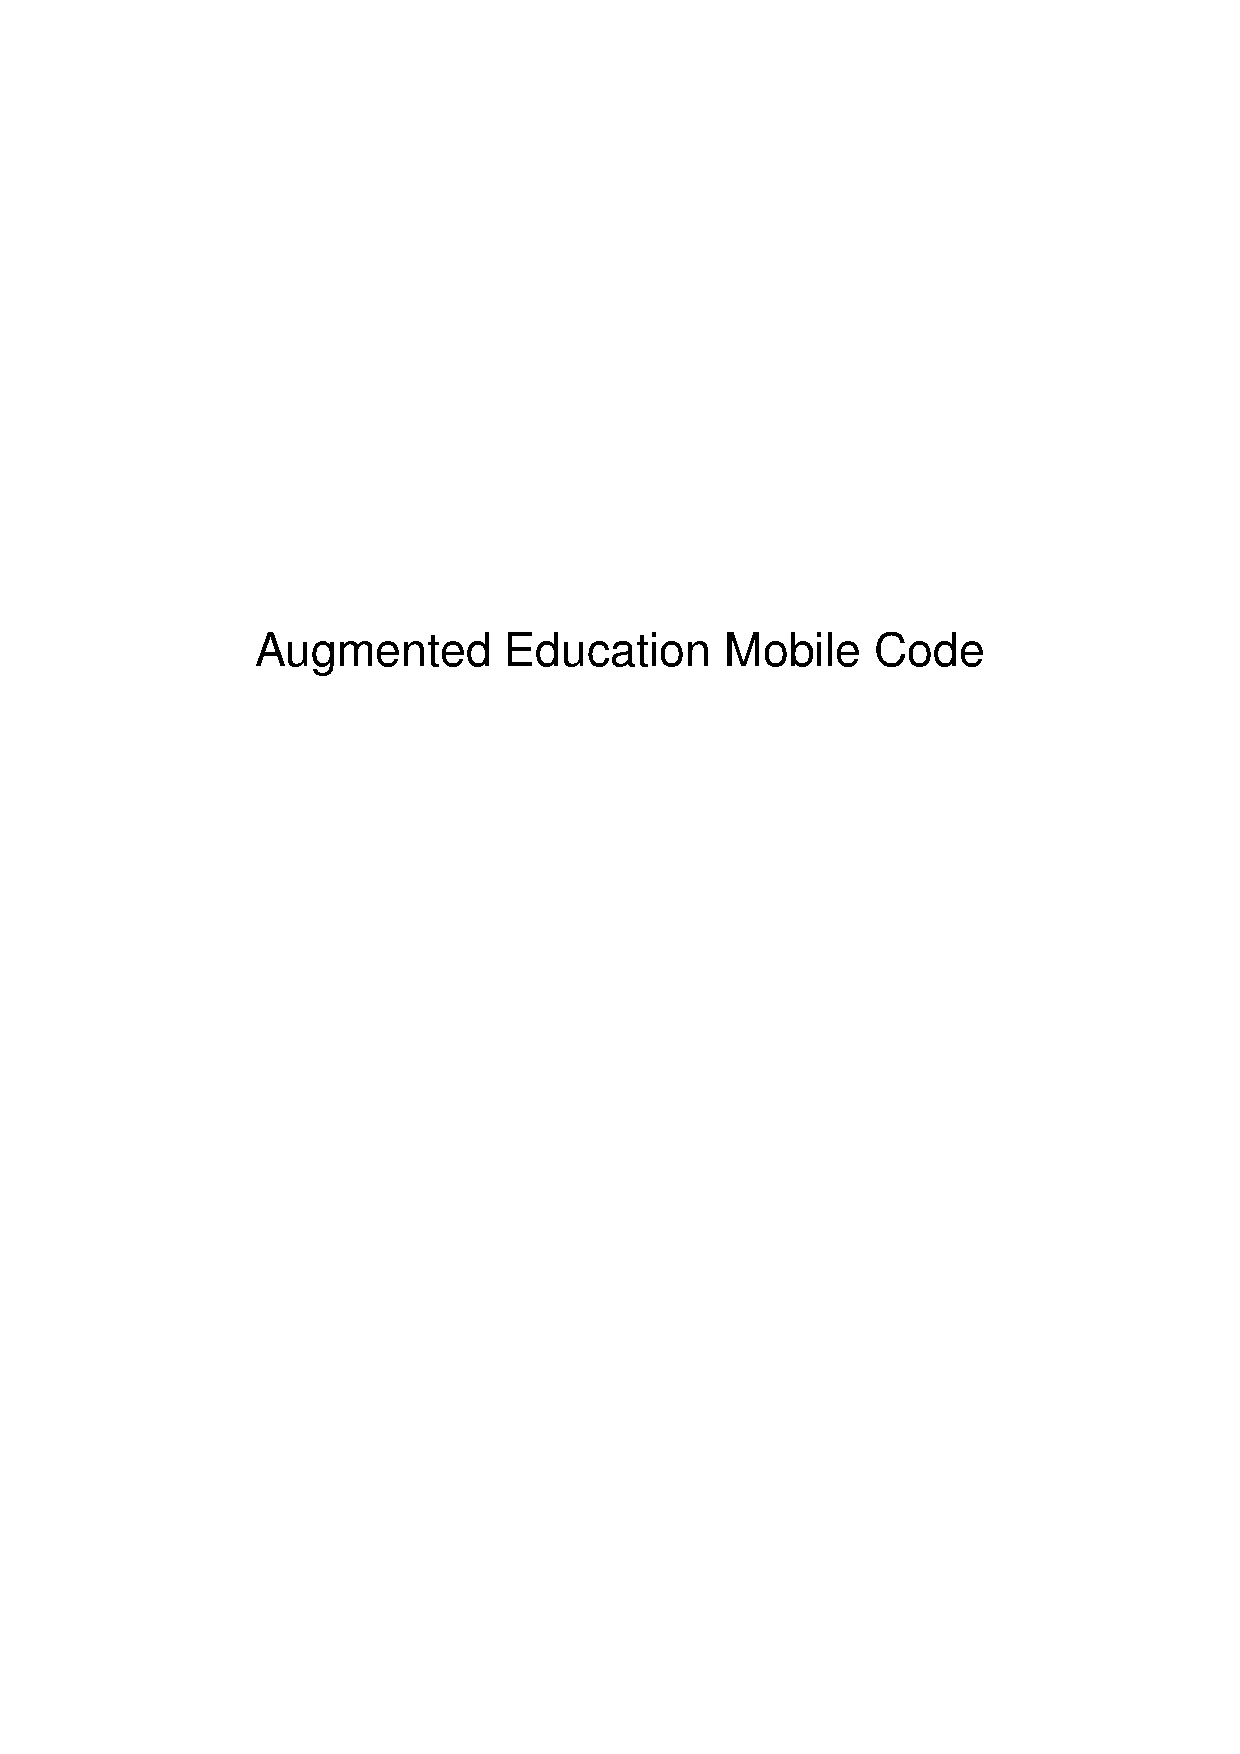
\includepdf[pages={1}, pagecommand=\section{Mobile Application}]{CodeDocumentation/MobileCodeDoc}
\includepdf[pages={2-}]{CodeDocumentation/MobileCodeDoc}